\documentclass[10pt, a4paper]{article}
\usepackage{latexsym}
\usepackage{amssymb,amsmath}
\usepackage[pdftex]{graphicx}
\newcommand{\dbar}[1]{\Bar{\Bar{#1}}}

\topmargin = 0.1in \textwidth=5.7in \textheight=8.6in

\oddsidemargin = 0.1in \evensidemargin = 0.1in

% headers
\usepackage{fancyhdr}
\usepackage{bm}
\usepackage{subfigmat}
\usepackage{longtable}
\usepackage{booktabs}
\pagestyle{fancy}
\chead{} 
\rhead{\thepage} 
% footer
\lfoot{\small\scshape } 
\cfoot{} 
%%%% insert your name here %%%%
\rfoot{\footnotesize Author} 
\renewcommand{\headrulewidth}{.3pt} 
\renewcommand{\footrulewidth}{.3pt}
\setlength\voffset{-0.25in}
\setlength\textheight{648pt}

\begin{document}

\title{Weissinger Vortex Lifting Line as a GP}
\author{Michael Burton}
\maketitle

This write-up is an attempt to formulate the Weissinger Vortex Lifting Line method as a geometric program (GP).  
With little modification this method can be cast as a signomial program (SP).  
However, formulation as a GP is not as straightforward.  
This write-up attempts to explain why this method is not GP-compatible even though it is convex. 
One approach to formulate this method as a GP is presented so that new insights might be had in solving this problem. 

\section*{Weissinger Vortex Lifting Line}

The Weissinger Vortex Lifting Line (WVL) is a lifting line method used to predict aerodynamic forces on a lifting surface.  It uses a collection of horseshoe vortex filaments along the span, each h.v.\ filament having constant strength $\Gamma_i$. 
A derivation of the WVL will not be given in this write-up as it is well documented elsewhere and follows the same principles of a vortex lattice method. 
The equations for the parameters of interest, coefficient of lift $C_L$ and coefficient of induced drag $C_{D_i}$, are 

\begin{align}
    \label{e:cl}
    C_L &= 2 \bar{\Gamma}^{\mathrm{T}} (\bar{V}_x \vec{\Delta y})/S_{\mathrm{ref}} \\
    &= \frac{2}{S_{\mathrm{ref}}} (\bar{\Gamma}_1 \bar{V}_{x_1} \Delta y_1 + \bar{\Gamma}_2 \bar{V}_{x_2} \Delta y_2 + \dots + \bar{\Gamma}_N \bar{V}_{x_N} \Delta y_N) \nonumber \\
    \label{e:cdi}
    C_{D_i} &= 2 \bar{\Gamma}^{\mathrm{T}} \bar{\bar{B}} \bar{\Gamma}/S_{\mathrm{ref}} \\
            &= \frac{2}{S_{\mathrm{ref}}} (B_{1,1} \Gamma_1^2 + B_{1,2} \Gamma_1 \Gamma_2 + B_{1,3}\Gamma_1 \Gamma_3 + \dots + B_{N,N} \Gamma_N^2) \nonumber
\end{align}
where the normalized h.v.\ filament strength is $ \bar{\Gamma} = \Gamma/V_{\inf}$, and the local normalized x-component of the velocity is $\bar{V}_x = u/V_{\inf}$.
The h.v.\ filaments can be distributed along the span in a cosine distribution as shown in Figure~\ref{f:wvl}.  

\begin{figure}[h!]
	\begin{center}
	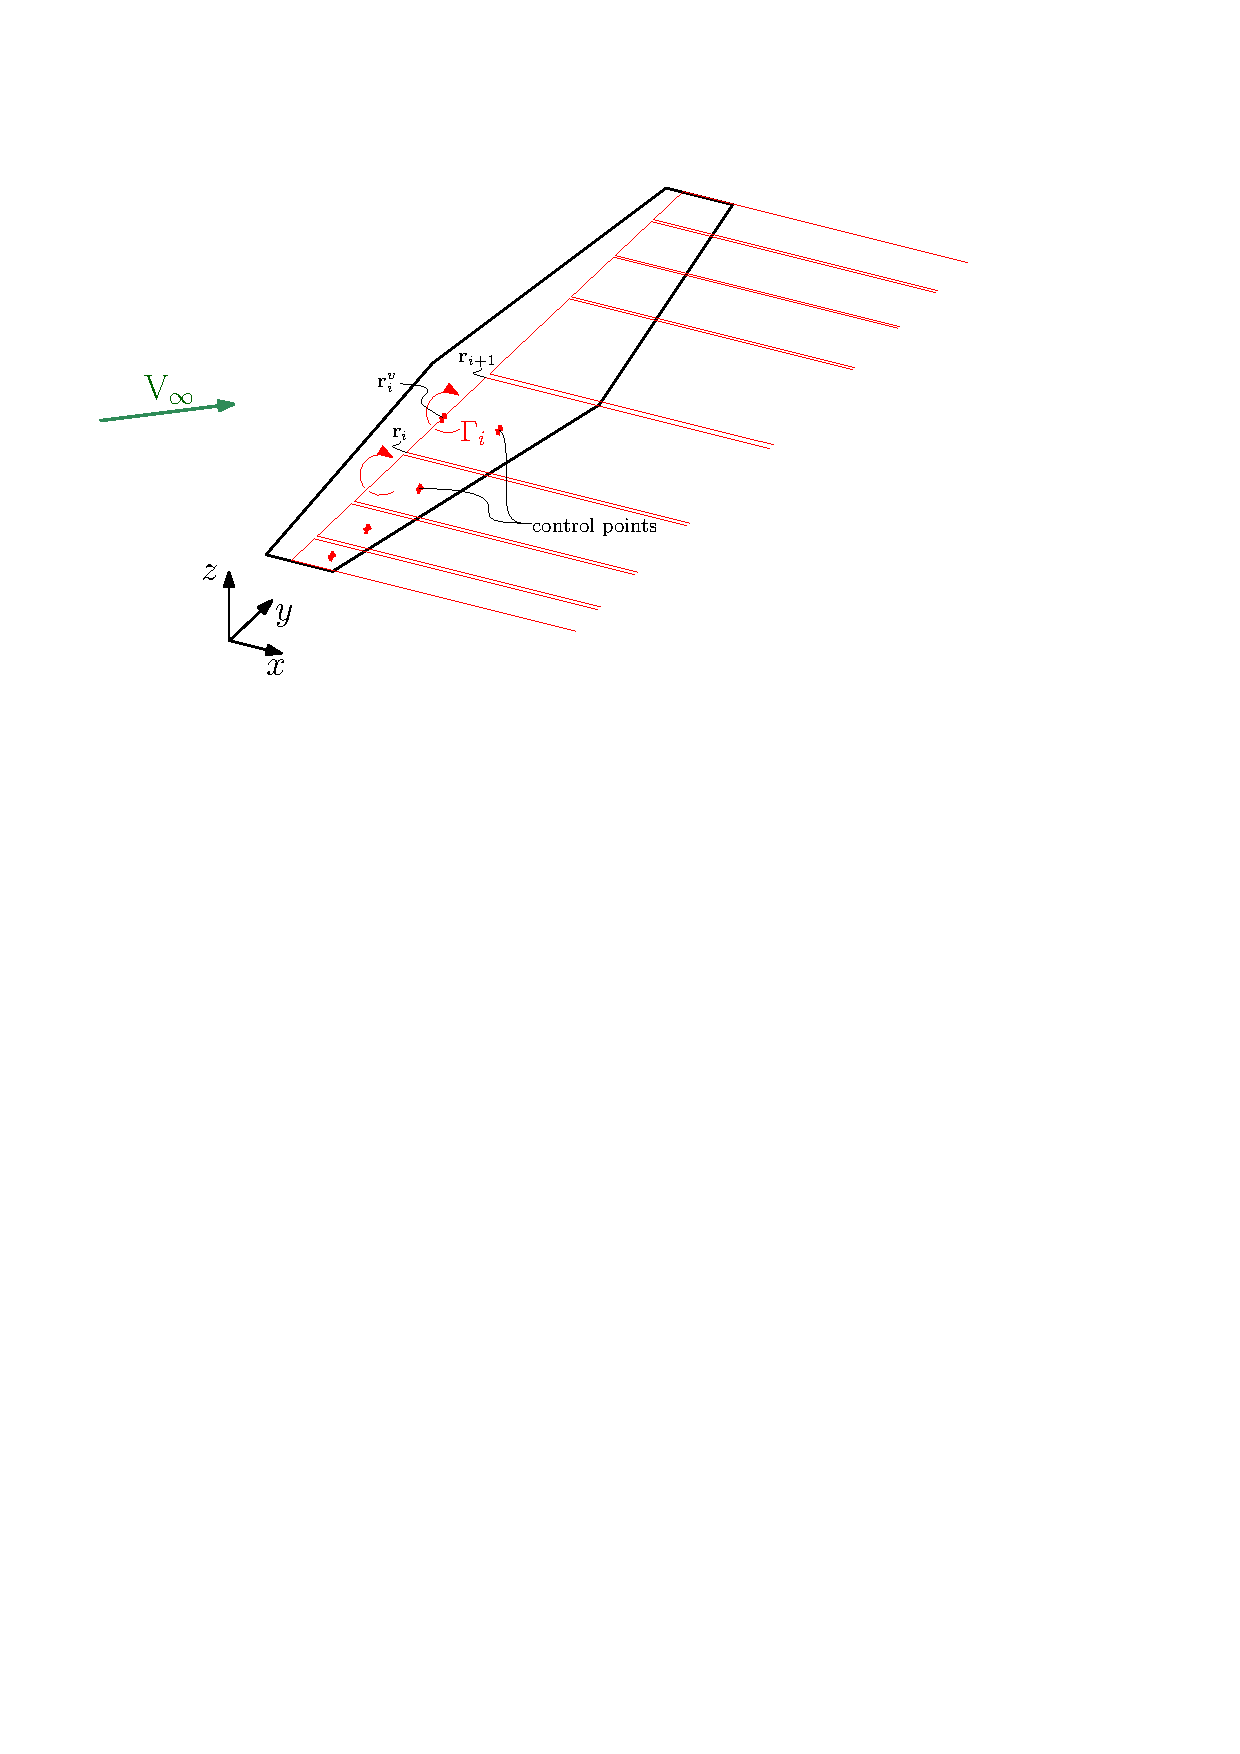
\includegraphics[width=0.8\textwidth]{wvl.pdf}
    \caption{Cosine distribution of h.v.\ filaments on constant taper wing.}
	\label{f:wvl}
	\end{center}
\end{figure}

The h.v.\ filament strength $\Gamma$, is related to the physical geometry through the Aerodynamic Influence Coefficient (AIC) matrix $A$, 

\begin{equation}
    \bar{\bar{A}} \bar{\Gamma} = \bar{\mathbf{U}}
\end{equation}
where $\bar{\mathbf{U}}$ is the local normalized velocity vector. The AIC matrix is defined as 

\begin{align}
    A_{ij} &\equiv \hat{\mathbf{V}}_j (\mathbf{r}_i^c) \cdot \bm{n}_{0_i} \\
    \hat{\mathbf{V}}_i (\mathbf{r}) &= \frac{1}{4\pi} \left[ \frac{\mathbf{a} \times \mathbf{b}}{|\mathbf{a}| |\mathbf{b}| + \mathbf{a} \cdot \mathbf{b}} \left( \frac{1}{|\mathbf{a}|} + \frac{1}{|\mathbf{b}|}\right) + \frac{\mathbf{a} \times \hat{\mathbf{x}}}{|\mathbf{a}| - \mathbf{a} \cdot \hat{\mathbf{x}}} \frac{1}{|\mathbf{a}|} - \frac{\mathbf{b} \times \hat{\mathbf{x}}}{|\mathbf{b}| - \mathbf{b} \cdot \hat{\mathbf{x}}} \frac{1}{|\mathbf{b}|} \right]
\end{align}

where the vectors $\bm{\mathrm{a}}$, $\bm{\mathrm{b}}$, and $\bm{\mathrm{x}}$ are defined in Figure~\ref{f:singlehv}. The control vector $\bm{\mathrm{r}}_i^c$ is defined in Figure~\ref{f:singlecp}. 
The WVL method assumes the control vector $\bm{\mathrm{r}}_i^c$ to be a vector to the three-quarters chord $\frac{3}{4}c$.  
The unit normal vector $\bm{n}_{0_i}$, can be approximated as a function of the local twist

\begin{equation}
    \bm{n}_{0_i} \approx \sin{\theta_i} \hat{x} + \cos{\theta_i} \hat{z}
\end{equation}

\begin{figure}[h!]
 \begin{subfigmatrix}{2}% number of columns
     \subfigure[$\bm{\mathrm{a}}$, $\bm{\mathrm{b}}$, and $\bm{\mathrm{x}}$ vector definition \label{f:singlehv}]{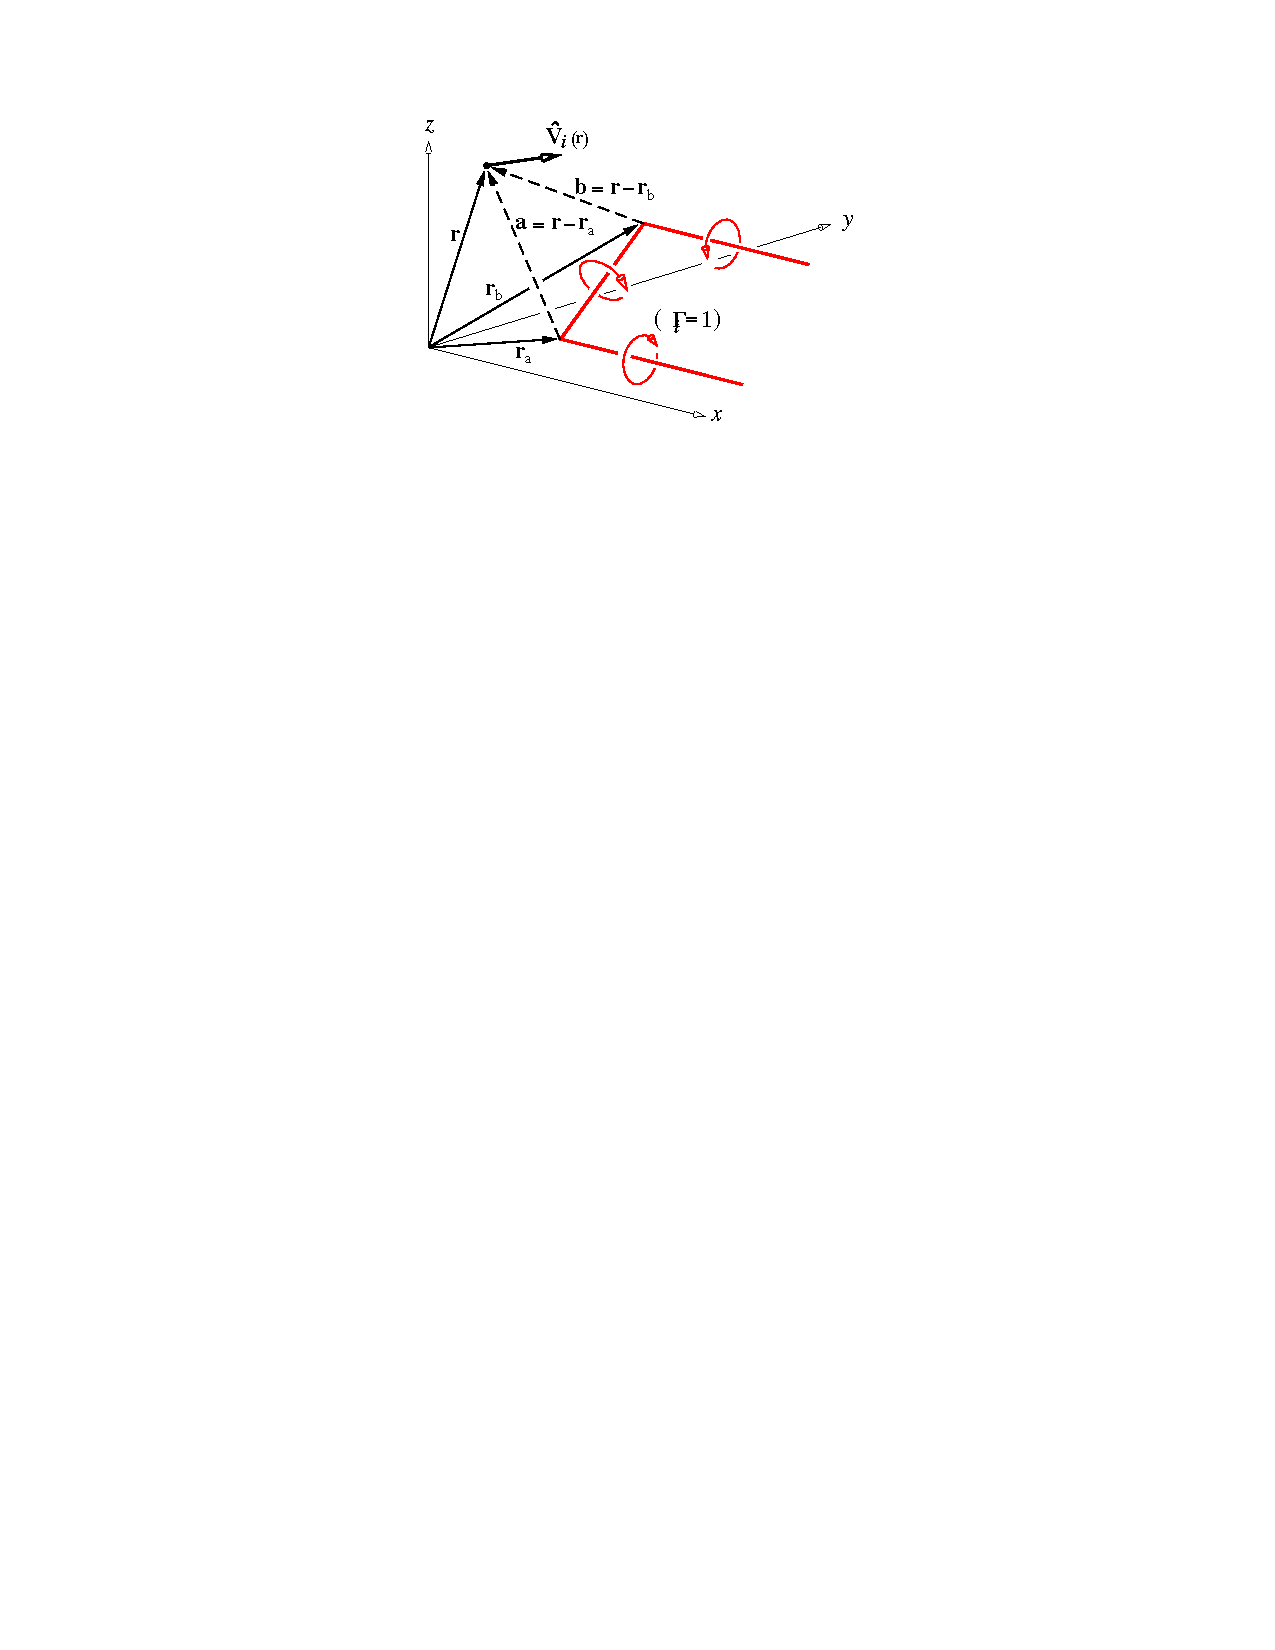
\includegraphics{singlehv.pdf}}
     \subfigure[Control vector $\bm{\mathrm{r}}_i^c$ definition \label{f:singlecp}]{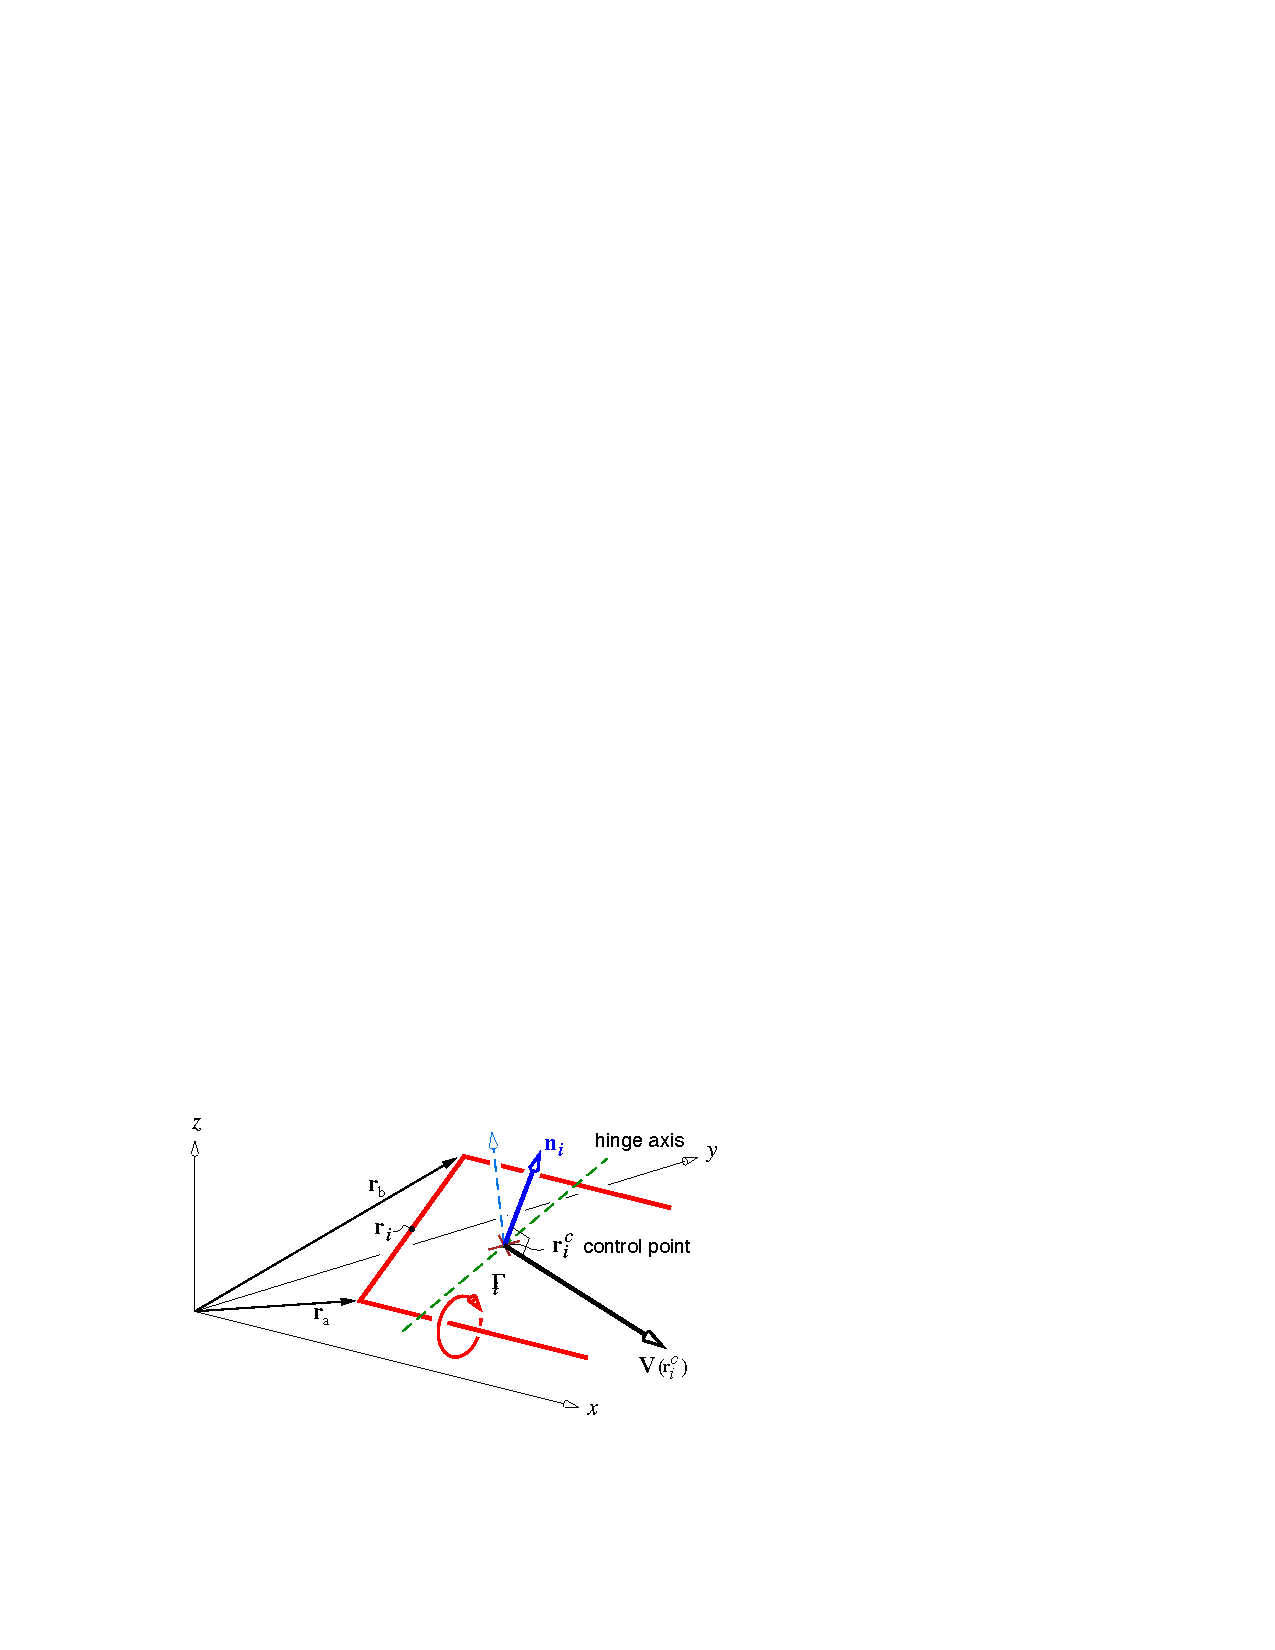
\includegraphics{singlecp.pdf}}
 \end{subfigmatrix}
 \caption{Geometry of one horseshoe vortex.}
 \label{f:singlevortex}
\end{figure}

The $\bar{\bar{B}}$ matrix, also a function of the geometry, depends on the vortex midpoint $\mathbf{r}_i^v$, not the control point $\mathbf{r}_i^c$

\begin{align}
    B_{ij} &= \frac{\Delta y_i}{4\pi} \left[ \frac{y_i^v - y_i}{(y_i^v - y_i)^2 + (z_i^v - z_i)^2} - \frac{y_i^v - y_{i+1}}{(y_i^v - y_{i+1})^2 + (z_i^v - z_{i+1})^2} \right] \\
    &+ \frac{\Delta z_i}{4\pi} \left[ \frac{z_i^v - y_i}{(z_i^v - y_i)^2 + (z_i^v - z_i)^2} - \frac{z_i^v - z_{i+1}}{(y_i^v - y_{i+1})^2 + (z_i^v - z_{i+1})^2} \right] \nonumber
\end{align}

The system of equations can be solved using a Newton method and by specifying flow conditions such as a specified lift coefficient $C_{L_{\mathrm{spec}}}$.

% \begin{figure}[h!]
% 	\begin{center}
% 	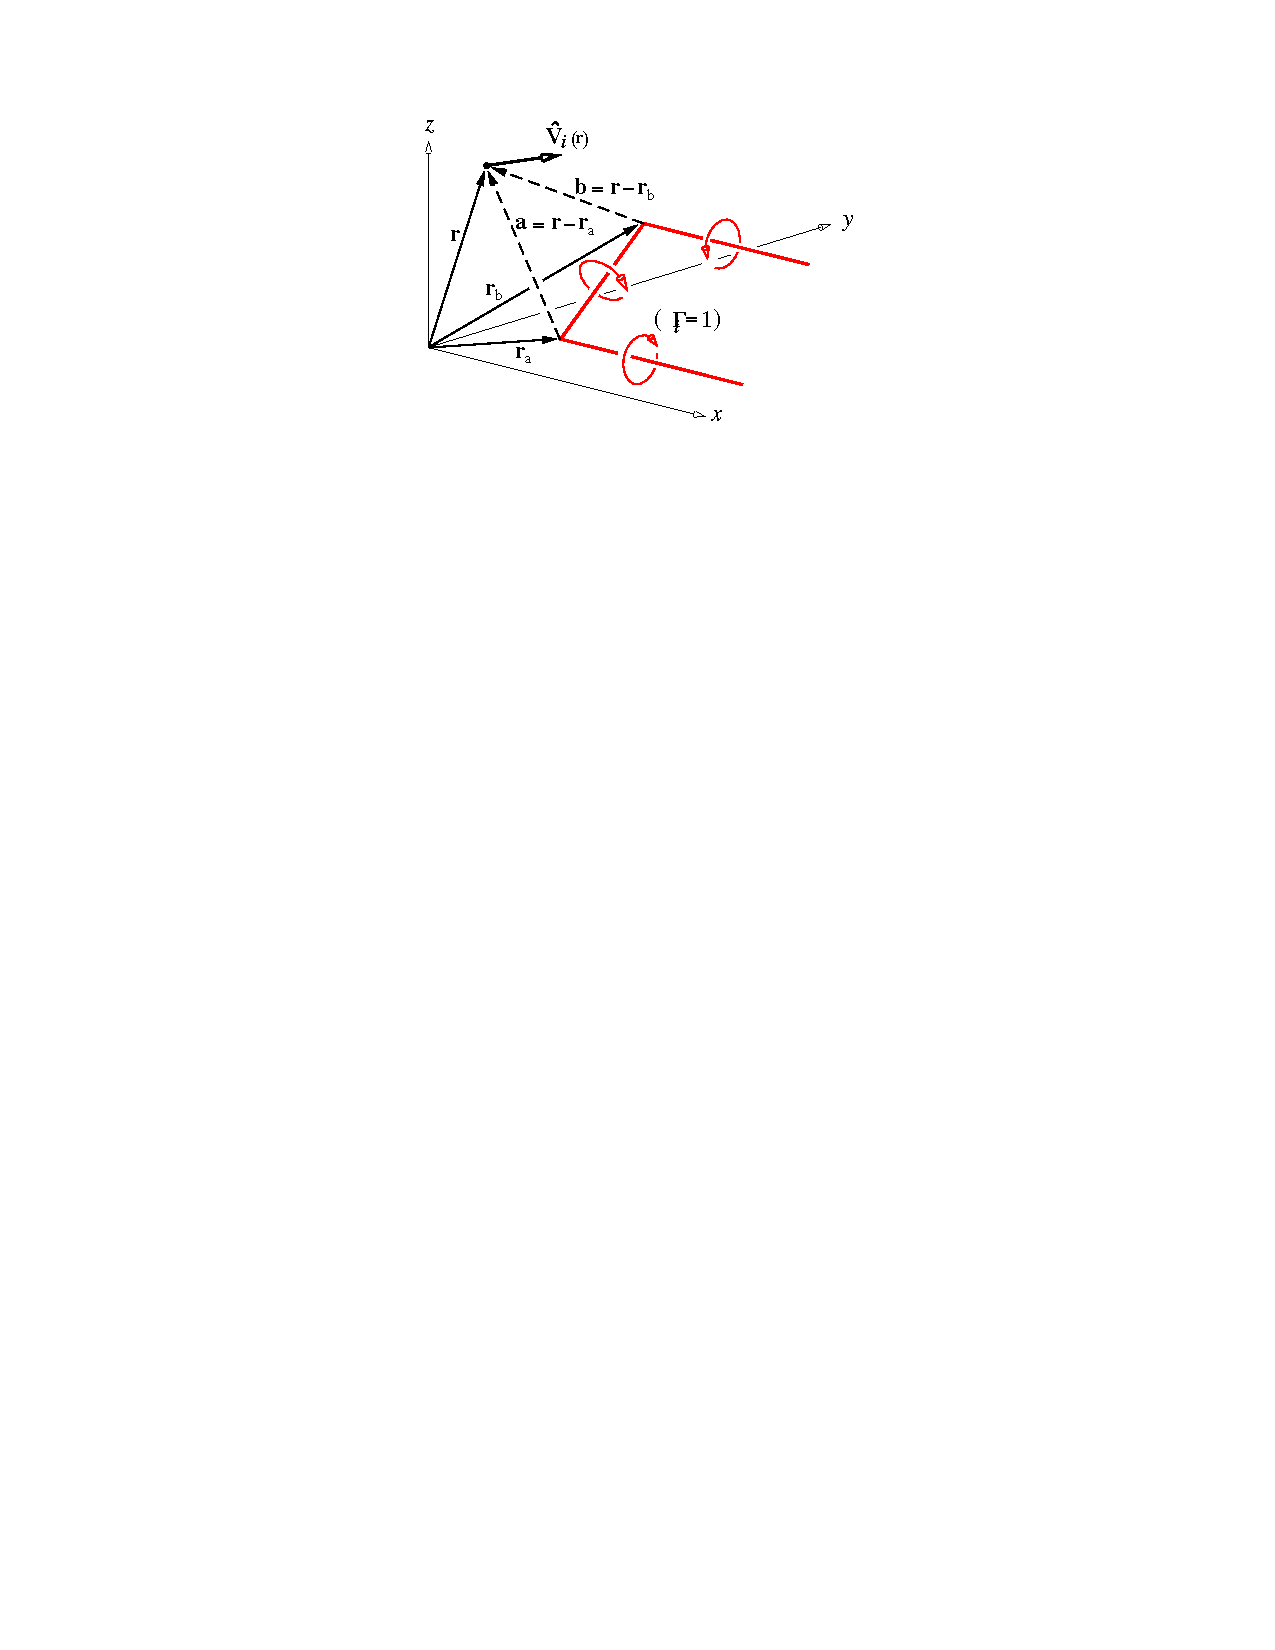
\includegraphics[width=0.6\textwidth]{singlehv.pdf}
%     \caption{Geometry of one horseshoe vortex.}
% 	\label{f:singlehv}
% 	\end{center}
% \end{figure}

\section{WVL as a GP: Problem Set Up}

Geometric programs are non-linear optimization problems with a particlar form

\begin{alignat*}{3}
    \text{minimize }\quad & g_0 (x) && \\
    \text{subject to }\quad & f_i(x) &= 1,\quad  i&=1,\dots,m \\
                            & g_i(x) &\leq 1, \quad i&=1,\dots,n 
\end{alignat*}
where monomials $f(x)$ and posynomials $g(x)$ are defined as

\begin{align}
    f(x) &= cx_1^{a_1}x_2^{a_2}  \dots x_n^{a_n}  \\
    g(x) &= \sum_{k=1}^K c_k x_1^{a_1k}x_2^{a_2k}  \dots x_n^{a_nk}
\end{align}

For the purposes of this exercise, it is assumed that the geometry is known.  
Specifically, all control vectors $\mathbf{r}_i^c$, node vectors $\mathbf{r}_i$, and midpoint vectors $\mathbf{r}_i^v$ are known.  Thus the AIC matrix $\bar{\bar{A}}$, and the $\bar{\bar{B}}$ matrix are also known.  
Futhermore, we will assume for now that $V_{x_i} = V_{\infty}$.  
Finally, the lift coefficient $C_L$, will be constrained by a specified number $C_{L_{\mathrm{spec}}}$ and the drag coefficient $C_{D_i}$ will be minimized.
This simplifies Equations~\ref{e:cl} and~\ref{e:cdi} to 

\begin{align}
    \label{e:clsp}
    C_{L_{\mathrm{spec}}} &= 2 \bar{\Gamma}^{\mathrm{T}} (\vec{\Delta y})/S_{\mathrm{ref}} \\
    \label{e:cdsp}
    C_{D_i} &= 2 \bar{\Gamma}^{\mathrm{T}} \bar{\bar{B}} \bar{\Gamma}/S_{\mathrm{ref}} 
\end{align}
Because the geometry is known, this problem can be adequately defined by these two equations. 

At first glance, Equations~\ref{e:clsp} and~\ref{e:cdsp} both seem like posynomials.  
If this were the case, the problem would be solved and we could stop here.  
However, a closer look at the upper and lower variable bounds reveals this is not the case. 

For a GP to be well defined, each variable must have an upper or lower bound.
A variable with a value, is called a fixed variable and is both upper and lower bounded by the assigned value.  
A maximized variable is lower bounded by the objective function and a minimzed variable is upper bounded by the objective function. 
Every other variable must be upper and lower bounded by the constraints and direction of the inequalities.  

Because $C_{D_i}$ is being minimized and $C_{L_{\mathrm{spec}}}$ and $\bar{\bar{B}}$ are known, the only direction of inequalities that adequately upper and lower bounds each variable is

\begin{align}
    \text{minimize} & \quad C_{D_i} \nonumber \\
    \label{e:cleq}
    C_{L_{\mathrm{spec}}} &\leq 2 \bar{\Gamma}^{\mathrm{T}} (\vec{\Delta y})/S_{\mathrm{ref}} \\
    \label{e:cdeq}
    C_{D_i} &\geq 2 \bar{\Gamma}^{\mathrm{T}} \bar{\bar{B}} \bar{\Gamma}/S_{\mathrm{ref}}.
\end{align}
Table~\ref{t:bounds} shows every variable and lists its upper and lower bounds. 

\begin{longtable}{lcc}
\caption{Variable Boundedness}\\
\toprule
\toprule
\label{t:bounds}
Variable                    & Upper Bound       & Lower Bound      \\ \hline
$C_{L_{\mathrm{spec}}}$     & Value             & Value            \\
$C_{D_i}$                   & Objective         & Eq.~\ref{e:cdeq} \\
$\bar{\Gamma}_i$            & Eq.~\ref{e:cdeq}  & Eq.~\ref{e:cleq} \\
$B_{ij}$                    & Value             & Value            \\
$S_{\mathrm{ref}}$          & Value             & Value            \\
\bottomrule
\end{longtable}

Unfortuantely, this formulation is not GP-compatible because Equation~\ref{e:cleq} is not posynomial.  
A general rule of thumb for GP compatibility is that sums of ``bad'' things are GP compatible and sums of ``good'' things are not.  
For example, weight is usually a negative thing for aircraft.  Therefore, a weight summation $W_{\mathrm{total}} \geq \sum W_i$ is usually GP compatible. 
In this case, we have multiple h.v.\ filaments that each provide some lift.  
From a very simplistic standpoint, the solver cannot correctly optimize the $\Gamma$ values because it only sees each $\Gamma$ as wanting more because lift is a good thing. 



\end{document}
